\section{Ti\-Xml\-Attribute Class Reference}
\label{classTiXmlAttribute}\index{TiXmlAttribute@{TiXmlAttribute}}
An attribute is a name-value pair.  


{\tt \#include $<$tinyxml.h$>$}

Inheritance diagram for Ti\-Xml\-Attribute::\begin{figure}[H]
\begin{center}
\leavevmode
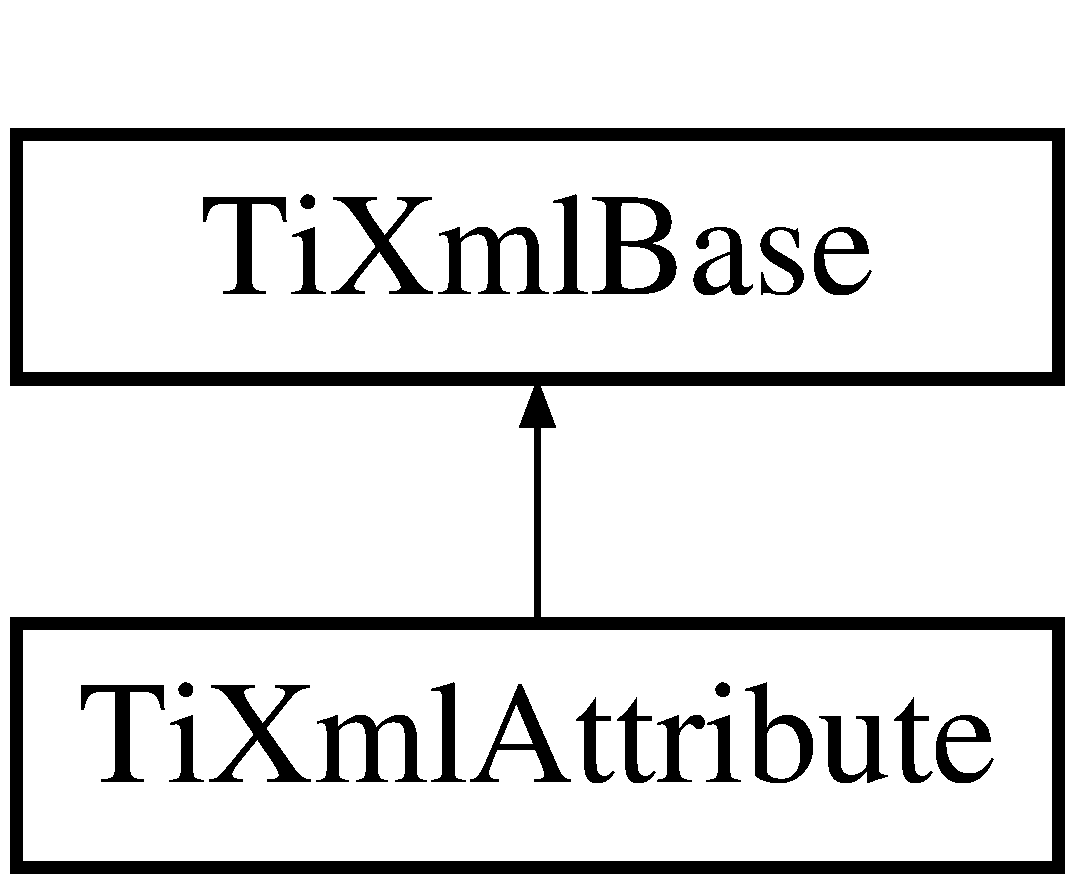
\includegraphics[height=2cm]{classTiXmlAttribute}
\end{center}
\end{figure}
\subsection*{Public Types}
\begin{CompactItemize}
\item 
enum \{ \par
{\bf TIXML\_\-NO\_\-ERROR} =  0, 
{\bf TIXML\_\-ERROR}, 
{\bf TIXML\_\-ERROR\_\-OPENING\_\-FILE}, 
{\bf TIXML\_\-ERROR\_\-OUT\_\-OF\_\-MEMORY}, 
\par
{\bf TIXML\_\-ERROR\_\-PARSING\_\-ELEMENT}, 
{\bf TIXML\_\-ERROR\_\-FAILED\_\-TO\_\-READ\_\-ELEMENT\_\-NAME}, 
{\bf TIXML\_\-ERROR\_\-READING\_\-ELEMENT\_\-VALUE}, 
{\bf TIXML\_\-ERROR\_\-READING\_\-ATTRIBUTES}, 
\par
{\bf TIXML\_\-ERROR\_\-PARSING\_\-EMPTY}, 
{\bf TIXML\_\-ERROR\_\-READING\_\-END\_\-TAG}, 
{\bf TIXML\_\-ERROR\_\-PARSING\_\-UNKNOWN}, 
{\bf TIXML\_\-ERROR\_\-PARSING\_\-COMMENT}, 
\par
{\bf TIXML\_\-ERROR\_\-PARSING\_\-DECLARATION}, 
{\bf TIXML\_\-ERROR\_\-DOCUMENT\_\-EMPTY}, 
{\bf TIXML\_\-ERROR\_\-EMBEDDED\_\-NULL}, 
{\bf TIXML\_\-ERROR\_\-PARSING\_\-CDATA}, 
\par
{\bf TIXML\_\-ERROR\_\-STRING\_\-COUNT}
 \}
\end{CompactItemize}
\subsection*{Public Member Functions}
\begin{CompactItemize}
\item 
{\bf Ti\-Xml\-Attribute} ()\label{classTiXmlAttribute_TiXmlAttributea0}

\begin{CompactList}\small\item\em Construct an empty attribute. \item\end{CompactList}\item 
{\bf Ti\-Xml\-Attribute} (const std::string \&\_\-name, const std::string \&\_\-value)\label{classTiXmlAttribute_TiXmlAttributea1}

\begin{CompactList}\small\item\em std::string constructor. \item\end{CompactList}\item 
{\bf Ti\-Xml\-Attribute} (const char $\ast$\_\-name, const char $\ast$\_\-value)\label{classTiXmlAttribute_TiXmlAttributea2}

\begin{CompactList}\small\item\em Construct an attribute with a name and value. \item\end{CompactList}\item 
const char $\ast$ {\bf Name} () const\label{classTiXmlAttribute_TiXmlAttributea3}

\begin{CompactList}\small\item\em Return the name of this attribute. \item\end{CompactList}\item 
const char $\ast$ {\bf Value} () const\label{classTiXmlAttribute_TiXmlAttributea4}

\begin{CompactList}\small\item\em Return the value of this attribute. \item\end{CompactList}\item 
int {\bf Int\-Value} () const\label{classTiXmlAttribute_TiXmlAttributea5}

\begin{CompactList}\small\item\em Return the value of this attribute, converted to an integer. \item\end{CompactList}\item 
double {\bf Double\-Value} () const\label{classTiXmlAttribute_TiXmlAttributea6}

\begin{CompactList}\small\item\em Return the value of this attribute, converted to a double. \item\end{CompactList}\item 
int {\bf Query\-Int\-Value} (int $\ast$\_\-value) const
\begin{CompactList}\small\item\em Query\-Int\-Value examines the value string. \item\end{CompactList}\item 
int {\bf Query\-Double\-Value} (double $\ast$\_\-value) const\label{classTiXmlAttribute_TiXmlAttributea8}

\begin{CompactList}\small\item\em Query\-Double\-Value examines the value string. See {\bf Query\-Int\-Value()}{\rm (p.\,\pageref{classTiXmlAttribute_TiXmlAttributea7})}. \item\end{CompactList}\item 
void {\bf Set\-Name} (const char $\ast$\_\-name)\label{classTiXmlAttribute_TiXmlAttributea9}

\begin{CompactList}\small\item\em Set the name of this attribute. \item\end{CompactList}\item 
void {\bf Set\-Value} (const char $\ast$\_\-value)\label{classTiXmlAttribute_TiXmlAttributea10}

\begin{CompactList}\small\item\em Set the value. \item\end{CompactList}\item 
void {\bf Set\-Int\-Value} (int \_\-value)\label{classTiXmlAttribute_TiXmlAttributea11}

\begin{CompactList}\small\item\em Set the value from an integer. \item\end{CompactList}\item 
void {\bf Set\-Double\-Value} (double \_\-value)\label{classTiXmlAttribute_TiXmlAttributea12}

\begin{CompactList}\small\item\em Set the value from a double. \item\end{CompactList}\item 
void {\bf Set\-Name} (const std::string \&\_\-name)\label{classTiXmlAttribute_TiXmlAttributea13}

\begin{CompactList}\small\item\em STL std::string form. \item\end{CompactList}\item 
void {\bf Set\-Value} (const std::string \&\_\-value)\label{classTiXmlAttribute_TiXmlAttributea14}

\begin{CompactList}\small\item\em STL std::string form. \item\end{CompactList}\item 
const {\bf Ti\-Xml\-Attribute} $\ast$ {\bf Next} () const\label{classTiXmlAttribute_TiXmlAttributea15}

\begin{CompactList}\small\item\em Get the next sibling attribute in the DOM. Returns null at end. \item\end{CompactList}\item 
{\bf Ti\-Xml\-Attribute} $\ast$ {\bf Next} ()\label{classTiXmlAttribute_TiXmlAttributea16}

\item 
const {\bf Ti\-Xml\-Attribute} $\ast$ {\bf Previous} () const\label{classTiXmlAttribute_TiXmlAttributea17}

\begin{CompactList}\small\item\em Get the previous sibling attribute in the DOM. Returns null at beginning. \item\end{CompactList}\item 
{\bf Ti\-Xml\-Attribute} $\ast$ {\bf Previous} ()\label{classTiXmlAttribute_TiXmlAttributea18}

\item 
bool {\bf operator==} (const {\bf Ti\-Xml\-Attribute} \&rhs) const\label{classTiXmlAttribute_TiXmlAttributea19}

\item 
bool {\bf operator$<$} (const {\bf Ti\-Xml\-Attribute} \&rhs) const\label{classTiXmlAttribute_TiXmlAttributea20}

\item 
bool {\bf operator$>$} (const {\bf Ti\-Xml\-Attribute} \&rhs) const\label{classTiXmlAttribute_TiXmlAttributea21}

\item 
virtual const char $\ast$ {\bf Parse} (const char $\ast$p, Ti\-Xml\-Parsing\-Data $\ast$data, Ti\-Xml\-Encoding encoding)\label{classTiXmlAttribute_TiXmlAttributea22}

\item 
virtual void {\bf Print} (FILE $\ast$cfile, int depth) const
\begin{CompactList}\small\item\em All Tiny\-Xml classes can print themselves to a filestream. \item\end{CompactList}\item 
virtual void {\bf Stream\-Out} (TIXML\_\-OSTREAM $\ast$out) const\label{classTiXmlAttribute_TiXmlAttributea24}

\item 
void {\bf Set\-Document} ({\bf Ti\-Xml\-Document} $\ast$doc)\label{classTiXmlAttribute_TiXmlAttributea25}

\item 
int {\bf Row} () const
\begin{CompactList}\small\item\em Return the position, in the original source file, of this node or attribute. \item\end{CompactList}\item 
int {\bf Column} () const\label{classTiXmlBase_TiXmlUnknowna79}

\begin{CompactList}\small\item\em See {\bf Row()}{\rm (p.\,\pageref{classTiXmlBase_TiXmlUnknowna78})}. \item\end{CompactList}\item 
void {\bf Set\-User\-Data} (void $\ast$user)\label{classTiXmlBase_TiXmlUnknowna80}

\item 
void $\ast$ {\bf Get\-User\-Data} ()\label{classTiXmlBase_TiXmlUnknowna81}

\end{CompactItemize}
\subsection*{Static Public Member Functions}
\begin{CompactItemize}
\item 
void {\bf Set\-Condense\-White\-Space} (bool condense)
\begin{CompactList}\small\item\em The world does not agree on whether white space should be kept or not. \item\end{CompactList}\item 
bool {\bf Is\-White\-Space\-Condensed} ()\label{classTiXmlBase_TiXmlUnknowne1}

\begin{CompactList}\small\item\em Return the current white space setting. \item\end{CompactList}\end{CompactItemize}
\subsection*{Static Public Attributes}
\begin{CompactItemize}
\item 
const int {\bf utf8Byte\-Table} [256]
\end{CompactItemize}
\subsection*{Static Protected Member Functions}
\begin{CompactItemize}
\item 
const char $\ast$ {\bf Skip\-White\-Space} (const char $\ast$, Ti\-Xml\-Encoding encoding)\label{classTiXmlBase_TiXmlUnknownf0}

\item 
bool {\bf Is\-White\-Space} (char c)\label{classTiXmlBase_TiXmlUnknownf1}

\item 
bool {\bf Stream\-White\-Space} (TIXML\_\-ISTREAM $\ast$in, TIXML\_\-STRING $\ast$tag)\label{classTiXmlBase_TiXmlUnknownf2}

\item 
bool {\bf Stream\-To} (TIXML\_\-ISTREAM $\ast$in, int character, TIXML\_\-STRING $\ast$tag)\label{classTiXmlBase_TiXmlUnknownf3}

\item 
const char $\ast$ {\bf Read\-Name} (const char $\ast$p, TIXML\_\-STRING $\ast$name, Ti\-Xml\-Encoding encoding)\label{classTiXmlBase_TiXmlUnknownf4}

\item 
const char $\ast$ {\bf Read\-Text} (const char $\ast$in, TIXML\_\-STRING $\ast$text, bool ignore\-White\-Space, const char $\ast$end\-Tag, bool ignore\-Case, Ti\-Xml\-Encoding encoding)\label{classTiXmlBase_TiXmlUnknownf5}

\item 
const char $\ast$ {\bf Get\-Entity} (const char $\ast$in, char $\ast$value, int $\ast$length, Ti\-Xml\-Encoding encoding)\label{classTiXmlBase_TiXmlUnknownf6}

\item 
const char $\ast$ {\bf Get\-Char} (const char $\ast$p, char $\ast$\_\-value, int $\ast$length, Ti\-Xml\-Encoding encoding)\label{classTiXmlBase_TiXmlUnknownf7}

\item 
void {\bf Put\-String} (const TIXML\_\-STRING \&str, TIXML\_\-OSTREAM $\ast$out)\label{classTiXmlBase_TiXmlUnknownf8}

\item 
void {\bf Put\-String} (const TIXML\_\-STRING \&str, TIXML\_\-STRING $\ast$out)\label{classTiXmlBase_TiXmlUnknownf9}

\item 
bool {\bf String\-Equal} (const char $\ast$p, const char $\ast$end\-Tag, bool ignore\-Case, Ti\-Xml\-Encoding encoding)\label{classTiXmlBase_TiXmlUnknownf10}

\item 
int {\bf Is\-Alpha} (unsigned char any\-Byte, Ti\-Xml\-Encoding encoding)\label{classTiXmlBase_TiXmlUnknownf11}

\item 
int {\bf Is\-Alpha\-Num} (unsigned char any\-Byte, Ti\-Xml\-Encoding encoding)\label{classTiXmlBase_TiXmlUnknownf12}

\item 
int {\bf To\-Lower} (int v, Ti\-Xml\-Encoding encoding)\label{classTiXmlBase_TiXmlUnknownf13}

\item 
void {\bf Convert\-UTF32To\-UTF8} (unsigned long input, char $\ast$output, int $\ast$length)\label{classTiXmlBase_TiXmlUnknownf14}

\end{CompactItemize}
\subsection*{Protected Attributes}
\begin{CompactItemize}
\item 
Ti\-Xml\-Cursor {\bf location}\label{classTiXmlBase_TiXmlUnknownp7}

\item 
void $\ast$ {\bf user\-Data}\label{classTiXmlBase_TiXmlUnknownp8}

\begin{CompactList}\small\item\em Field containing a generic user pointer. \item\end{CompactList}\end{CompactItemize}
\subsection*{Static Protected Attributes}
\begin{CompactItemize}
\item 
const char $\ast$ {\bf error\-String} [TIXML\_\-ERROR\_\-STRING\_\-COUNT]
\end{CompactItemize}


\subsection{Detailed Description}
An attribute is a name-value pair. 

Elements have an arbitrary number of attributes, each with a unique name.

\begin{Desc}
\item[Note:]The attributes are not Ti\-Xml\-Nodes, since they are not part of the tiny\-XML document object model. There are other suggested ways to look at this problem. \end{Desc}




\subsection{Member Function Documentation}
\index{TiXmlAttribute@{Ti\-Xml\-Attribute}!Print@{Print}}
\index{Print@{Print}!TiXmlAttribute@{Ti\-Xml\-Attribute}}
\subsubsection{\setlength{\rightskip}{0pt plus 5cm}void Ti\-Xml\-Attribute::Print (FILE $\ast$ {\em cfile}, int {\em depth}) const\hspace{0.3cm}{\tt  [virtual]}}\label{classTiXmlAttribute_TiXmlAttributea23}


All Tiny\-Xml classes can print themselves to a filestream. 

This is a formatted print, and will insert tabs and newlines.

(For an unformatted stream, use the $<$$<$ operator.)

Implements {\bf Ti\-Xml\-Base} {\rm (p.\,\pageref{classTiXmlBase_TiXmlNodea73})}.

\index{TiXmlAttribute@{Ti\-Xml\-Attribute}!QueryIntValue@{QueryIntValue}}
\index{QueryIntValue@{QueryIntValue}!TiXmlAttribute@{Ti\-Xml\-Attribute}}
\subsubsection{\setlength{\rightskip}{0pt plus 5cm}int Ti\-Xml\-Attribute::Query\-Int\-Value (int $\ast$ {\em \_\-value}) const}\label{classTiXmlAttribute_TiXmlAttributea7}


Query\-Int\-Value examines the value string. 

It is an alternative to the {\bf Int\-Value()}{\rm (p.\,\pageref{classTiXmlAttribute_TiXmlAttributea5})} method with richer error checking. If the value is an integer, it is stored in 'value' and the call returns TIXML\_\-SUCCESS. If it is not an integer, it returns TIXML\_\-WRONG\_\-TYPE.

A specialized but useful call. Note that for success it returns 0, which is the opposite of almost all other Tiny\-Xml calls.\index{TiXmlAttribute@{Ti\-Xml\-Attribute}!Row@{Row}}
\index{Row@{Row}!TiXmlAttribute@{Ti\-Xml\-Attribute}}
\subsubsection{\setlength{\rightskip}{0pt plus 5cm}int Ti\-Xml\-Base::Row () const\hspace{0.3cm}{\tt  [inline, inherited]}}\label{classTiXmlBase_TiXmlUnknowna78}


Return the position, in the original source file, of this node or attribute. 

The row and column are 1-based. (That is the first row and first column is 1,1). If the returns values are 0 or less, then the parser does not have a row and column value.

Generally, the row and column value will be set when the Ti\-Xml\-Document::Load(), {\bf Ti\-Xml\-Document::Load\-File()}{\rm (p.\,\pageref{classTiXmlDocument_TiXmlDocumenta6})}, or any Ti\-Xml\-Node::Parse() is called. It will NOT be set when the DOM was created from operator$>$$>$.

The values reflect the initial load. Once the DOM is modified programmatically (by adding or changing nodes and attributes) the new values will NOT update to reflect changes in the document.

There is a minor performance cost to computing the row and column. Computation can be disabled if {\bf Ti\-Xml\-Document::Set\-Tab\-Size()}{\rm (p.\,\pageref{classTiXmlDocument_TiXmlDocumenta20})} is called with 0 as the value.

\begin{Desc}
\item[See also:]{\bf Ti\-Xml\-Document::Set\-Tab\-Size()}{\rm (p.\,\pageref{classTiXmlDocument_TiXmlDocumenta20})}\end{Desc}
\index{TiXmlAttribute@{Ti\-Xml\-Attribute}!SetCondenseWhiteSpace@{SetCondenseWhiteSpace}}
\index{SetCondenseWhiteSpace@{SetCondenseWhiteSpace}!TiXmlAttribute@{Ti\-Xml\-Attribute}}
\subsubsection{\setlength{\rightskip}{0pt plus 5cm}void Ti\-Xml\-Base::Set\-Condense\-White\-Space (bool {\em condense})\hspace{0.3cm}{\tt  [inline, static, inherited]}}\label{classTiXmlBase_TiXmlUnknowne0}


The world does not agree on whether white space should be kept or not. 

In order to make everyone happy, these global, static functions are provided to set whether or not Tiny\-Xml will condense all white space into a single space or not. The default is to condense. Note changing this values is not thread safe.

\subsection{Member Data Documentation}
\index{TiXmlAttribute@{Ti\-Xml\-Attribute}!errorString@{errorString}}
\index{errorString@{errorString}!TiXmlAttribute@{Ti\-Xml\-Attribute}}
\subsubsection{\setlength{\rightskip}{0pt plus 5cm}const char $\ast$ Ti\-Xml\-Base::error\-String\hspace{0.3cm}{\tt  [static, protected, inherited]}}\label{classTiXmlBase_TiXmlUnknownt0}


{\bf Initial value:}

\footnotesize\begin{verbatim}
{
    "No error",
    "Error",
    "Failed to open file",
    "Memory allocation failed.",
    "Error parsing Element.",
    "Failed to read Element name",
    "Error reading Element value.",
    "Error reading Attributes.",
    "Error: empty tag.",
    "Error reading end tag.",
    "Error parsing Unknown.",
    "Error parsing Comment.",
    "Error parsing Declaration.",
    "Error document empty.",
    "Error null (0) or unexpected EOF found in input stream.",
    "Error parsing CDATA.",
}
\end{verbatim}\normalsize 
\index{TiXmlAttribute@{Ti\-Xml\-Attribute}!utf8ByteTable@{utf8ByteTable}}
\index{utf8ByteTable@{utf8ByteTable}!TiXmlAttribute@{Ti\-Xml\-Attribute}}
\subsubsection{\setlength{\rightskip}{0pt plus 5cm}const int Ti\-Xml\-Base::utf8Byte\-Table\hspace{0.3cm}{\tt  [static, inherited]}}\label{classTiXmlBase_TiXmlUnknowns0}


{\bf Initial value:}

\footnotesize\begin{verbatim} 
{
    
        1,  1,  1,  1,  1,  1,  1,  1,  1,  1,  1,  1,  1,  1,  1,  1,  
        1,  1,  1,  1,  1,  1,  1,  1,  1,  1,  1,  1,  1,  1,  1,  1,  
        1,  1,  1,  1,  1,  1,  1,  1,  1,  1,  1,  1,  1,  1,  1,  1,  
        1,  1,  1,  1,  1,  1,  1,  1,  1,  1,  1,  1,  1,  1,  1,  1,  
        1,  1,  1,  1,  1,  1,  1,  1,  1,  1,  1,  1,  1,  1,  1,  1,  
        1,  1,  1,  1,  1,  1,  1,  1,  1,  1,  1,  1,  1,  1,  1,  1,  
        1,  1,  1,  1,  1,  1,  1,  1,  1,  1,  1,  1,  1,  1,  1,  1,  
        1,  1,  1,  1,  1,  1,  1,  1,  1,  1,  1,  1,  1,  1,  1,  1,  
        1,  1,  1,  1,  1,  1,  1,  1,  1,  1,  1,  1,  1,  1,  1,  1,  
        1,  1,  1,  1,  1,  1,  1,  1,  1,  1,  1,  1,  1,  1,  1,  1,  
        1,  1,  1,  1,  1,  1,  1,  1,  1,  1,  1,  1,  1,  1,  1,  1,  
        1,  1,  1,  1,  1,  1,  1,  1,  1,  1,  1,  1,  1,  1,  1,  1,  
        1,  1,  2,  2,  2,  2,  2,  2,  2,  2,  2,  2,  2,  2,  2,  2,  
        2,  2,  2,  2,  2,  2,  2,  2,  2,  2,  2,  2,  2,  2,  2,  2,  
        3,  3,  3,  3,  3,  3,  3,  3,  3,  3,  3,  3,  3,  3,  3,  3,  
        4,  4,  4,  4,  4,  1,  1,  1,  1,  1,  1,  1,  1,  1,  1,  1   
}
\end{verbatim}\normalsize 


The documentation for this class was generated from the following files:\begin{CompactItemize}
\item 
src/tinyxml.h\item 
src/tinyxml.cpp\item 
src/tinyxmlparser.cpp\end{CompactItemize}
